\chapter{Turnkey -- Piktotegner}
If you would like to work with an application that is essential to the creation of new pictograms, you should choose \textit{Piktotegner}.
\textit{Piktotegner} is an android application which provides a pictogram creation environment for tablets.
It is an application where the essential functionality to create pictograms is already established, but where usability improvement is needed.

When working on this application, we recommend performing several usability tests as well as stability testing, as there is some unclosed memory leaking issues.
Unit testing is also recommended, as none of this has been performed.

As of such, a GUI redesign is recommended, based on your performed usability tests and knowledge from the DEB course.

If you find that the application becomes well polished for the users' needs you can embark in a whole new part of the pictogram creation environment.
What is thought of here is a template environment, where you do not have to draw your own images, but can instead construct images from some predefined image structures, such as balls, stickmen, animals, machines and so forth, but where the user gets to choose the posture, colour theme, and accessories.

If you want to delve into how the elements of the image is drawn, rotated, and resized, be prepared for linear algebra, with rotation matrices, and euclidian geometry (taught in Advanced Algorithms).

\section{Application structure}
When launching the application, you start with the MainActivity.java. 
This is where all fragments and UI is launched from.

The drawing entities and their corresponding handlers are basically structured as seen in \figref{fig:turnkeydiacanvas}, and may need some restructuring.

\begin{figure}[h]
     \centering
     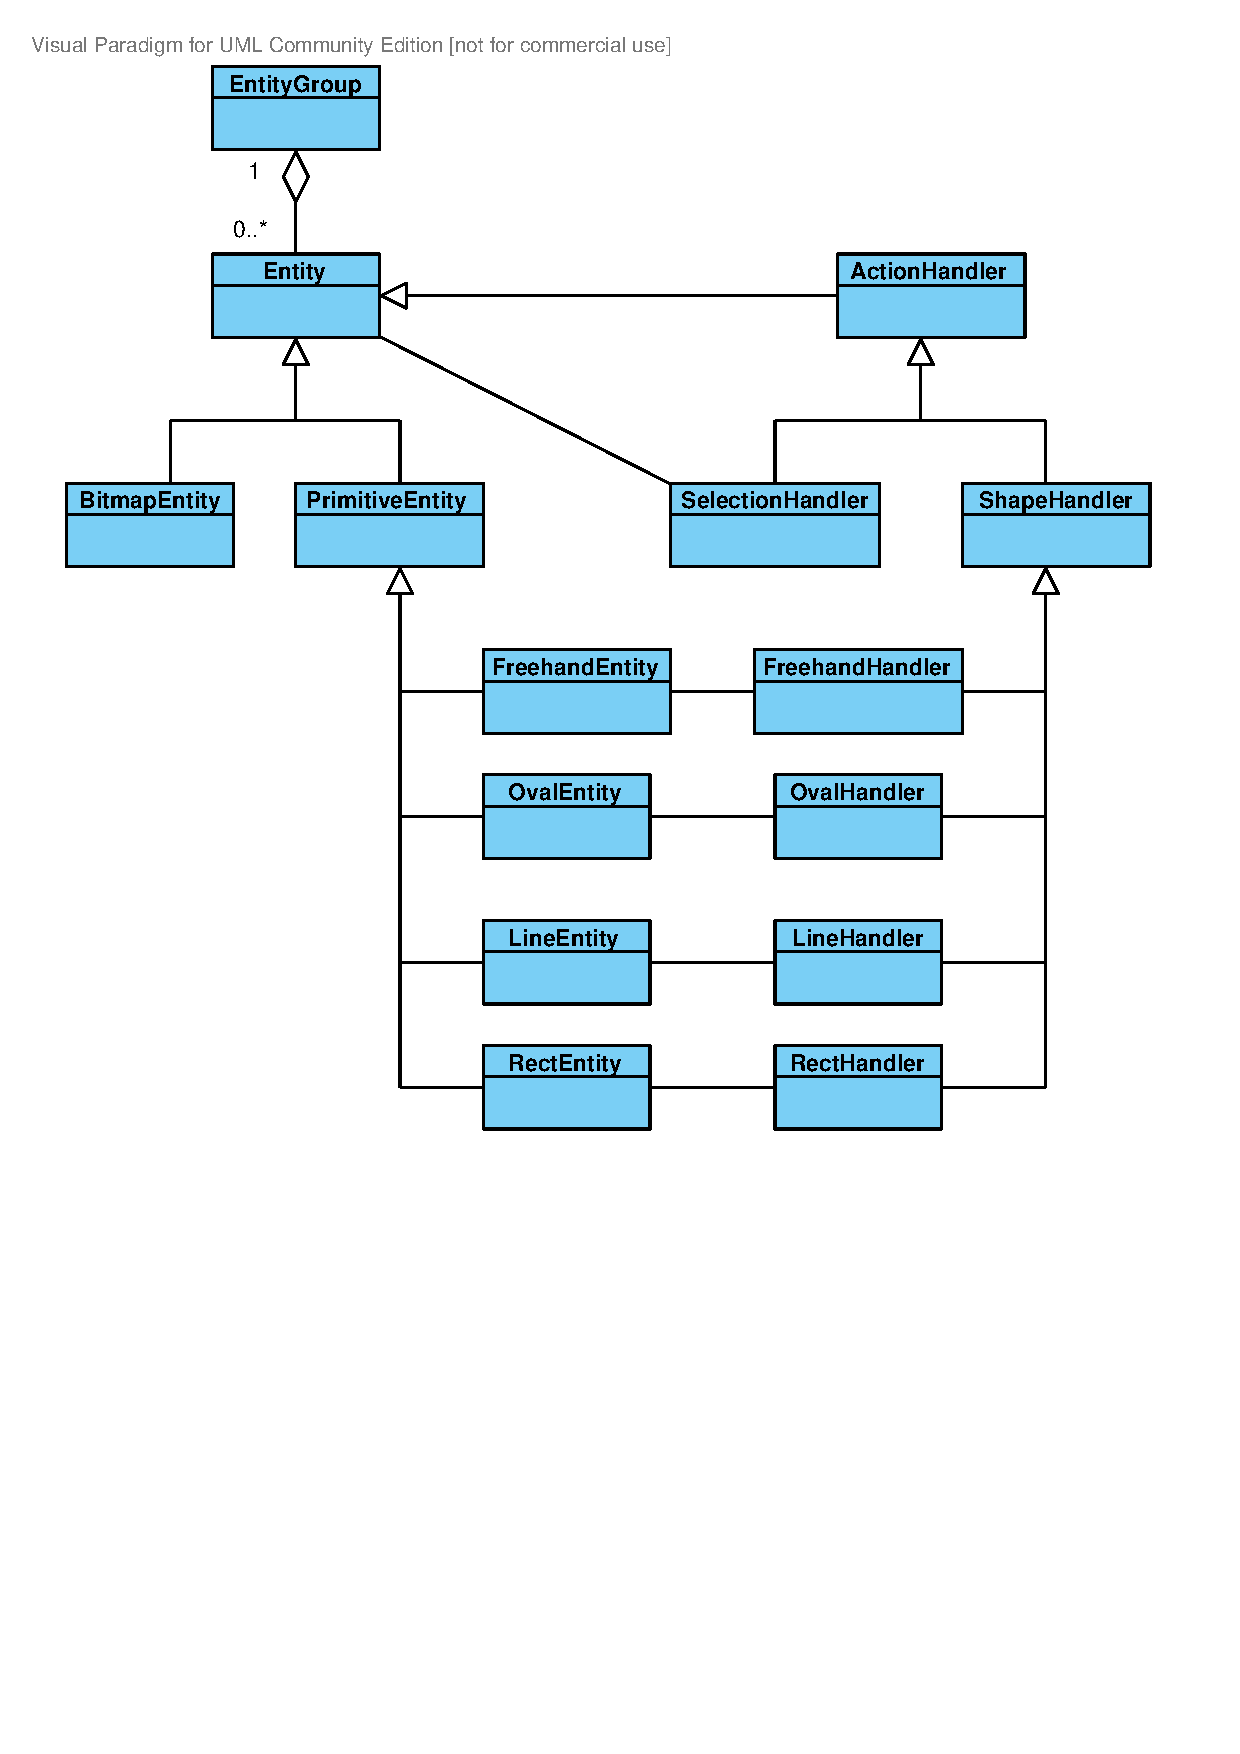
\includegraphics[trim= 1cm 10cm 1cm 1cm, clip, scale=0.5]{canvasdia-turnkey}
     \caption{Class Diagram with entities and handlers}
     \label{fig:turnkeydiacanvas}
\end{figure}

Apart from this, the application is structured into the mainActivity, which contatins a drawFragment, record dialogue, camera dialogue, save dialogue and help dialogue.
We recommend when you start to examine each class, as the code is well documented and in itself should serve as sufficient documentation.

Furthermore, we recommend Vogella's android tutorials, as they have been of great help throughout development.